\documentclass[tikz,border=10pt]{standalone}
\usetikzlibrary{calc}

\begin{document}
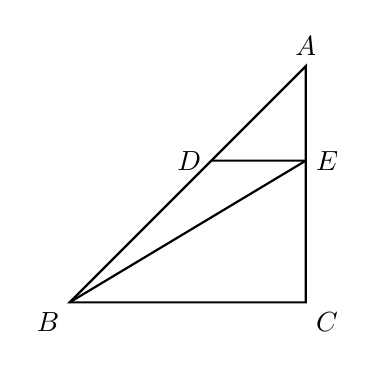
\begin{tikzpicture}[scale=1.5, thick]
    % 1. 定义坐标点
    \coordinate (C) at (0,0);
    \coordinate (B) at (-2,0);
    \coordinate (A) at (0,2);
    
    % 定义D点和E点 (D在AB上，E在AC上，满足DE平行BC)
    \coordinate (E) at (0, 1.2);
    \coordinate (D) at ($(B)!0.6!(A)$); % 通过插值定义D点位置

    % 2. 绘制主要三角形ABC
    \draw (A) -- (B) -- (C) -- cycle;
    
    % 3. 绘制内部辅助线
    \draw (D) -- (E); % 平行线
    \draw (B) -- (E); % 连接线BE

    % 4. 标注点位信息
    \node[above] at (A) {$A$};
    \node[below left] at (B) {$B$};
    \node[below right] at (C) {$C$};
    \node[left] at (D) {$D$};
    \node[right] at (E) {$E$};

\end{tikzpicture}
\end{document}